% puzzle
% theory cant explain 
% better theory 

% puzzle
Why do people comment on draft policies when they seem to have no new information to offer and no power to influence decisions? Who inspires them and to what end? 

Answering these questions requires a theory explaining variation in mass engagement.  
This section defines mass engagement and theorizes that we should observe different patterns of engagement depending on whether an organization launches a mobilization campaign as an outside lobbying tactic, to counter such a campaign, or for reasons other than influencing policy. In the next section, I develop methods to measure these patterns. In short, these measures capture similar statistics to questions posed by \citet[p. 9]{Verba1987}: ``How much participation is there, what kind is it, and from what segments of society does it come?'' I hypothesize that different segments of society have different reasons for participating and thus participated with different frequency and different types. 

% theory of IG influence 
A growing literature in political science draws on scholarship in law and public administration as well as studies of agenda setting and lobbying in legislative policymaking to better understand agencies as policymaking bodies. Public administration and legal scholars have been more attentive to the prominent role of interest groups. \citet{Kerwin2011} notes that ``Interest groups could find few modes of government decision making better suited to their particular strengths than rulemaking.'' This research finds business groups to be the most successful class of commenters in rulemaking \citep{Yackee2006JOP} especially when lobbying together, often, or unopposed \citep{Nelson2012} and when lobbying across multiple venues \citep{Yackee2015JPART}. Importantly, this literature notes that the currency of lobbying is information \citep{Hall2006, Carpenter1998, Yackee2006JPART, Yackee2012}, which includes both science and policy ideas \citep{Jones2005}. \citet{Kirilenko2014} and \citet{Yackee2006JOP} both find evidence that comments from sophisticated interest groups like businesses seem to influence rules. %These scholars offer one set of answers to the question of who wins: those who succeed in rulemaking tend to be business interests, repeat players, those who lobby together, and those who lobby unopposed. They 
\citet{Yackee2006JOP} theorize several mechanisms of influence, including bringing in new voices and sending unified messages at higher amplitudes, creating perceptions of political consensus.

% theory can't explain
However, as noted above, scholars of bureaucratic policymaking have focused on the sophisticated lobbying efforts of powerful interest groups such as business coalitions. A key insight from this scholarship is that technical information is the currency of insider lobbying. Figure \ref{fig:causal-classic-lobbying} illustrates the classic causal model of insider lobbying that describes most rulemakings. However, mass engagement has no place in this model. I aim to fill this gap.

% [INSERT - INFORMATION IS THE CURRENCY OF INTEREST GROUP LOBBYING]

\begin{figure}
    \centering
    \caption{The Classic Model of Interest Group Lobbying in Bureaucratic Policymaking}
    \label{fig:causal-classic-lobbying}
\tiny
\begin{tikzpicture}[%
    node distance=1.2cm,
    auto,
    text width=1.5cm,
dnode/.style={diamond, align=center, aspect=2, fill=green!5,draw=green!60, very thick, minimum size=2cm},
squarednode/.style={rectangle, align=center, aspect=1, draw=red!60, fill=red!5, very thick, minimum size=1cm},
pnode/.style={ellipse, align=center, aspect=1, draw=black!60, fill=black!5, very thick, minimum size=1cm},
title/.style={rectangle, align=center, aspect=1, minimum size=2cm},
]
% Draft 
\node[dnode]      (draft)                     {Draft Policy};



% Group Nodes
\node[pnode]      (groupdemands) [right=of draft] {Group Demands};
\node[dnode]        (groupdecides) [right=of groupdemands] {Lobbying};
\node[squarednode]      (groupinfo) [right=of groupdecides] {Technical Information};

% policy 
\node[dnode]      (policy)       [right=of groupinfo] {Policy Response};
\draw[->] (groupinfo.east) -- (policy.west);
% \draw[->] (publicinfo.east) -- (policy.west);
% \draw[->] (principalinfo.east) -- (policy.south);
% \draw[->] (principalinfo2.east) -- (policy.south);

% Group Lines
\draw[->] (draft.east) -- (groupdemands.west);
\draw[->] (groupdemands.east) -- (groupdecides.west);
\draw[->] (groupdecides.east) -- (groupinfo.west);

% Titles
% \node[title]      (1) [above=of draft] {Policy};
%\node[title]      (2) [above=of groupdemands] {Preferences};
%\node[title]      (4) [above=of groupinfo] {Information/ Signal};
%\node[title]      (3) [above=of groupdecides] {Observed Behavior};


\end{tikzpicture}
\end{figure}
\normalsize



% DEFINITION
\subsubsection{Defining mass engagement}
Political scientists often define civic engagement as writing to government officials, signing petitions, attending hearings, attending protests, or donate to a political campaign \citep{Verba1984}. While donating is more common in electoral politics, activists frequently target agency policymaking with letter-writing campaigns, petitions, hearings, and protests. 
% I suspect that mass commenting is driven by the same privileged populations known to engage in other civic activities. 
% Does it work? If so, by what mechanisms?

Following the conventional terms ``mass comment campaign'' and ``public engagement,'' I call the general phenomenon ``mass engagement'' resulting from a ``mass mobilization campaign'' in order to distinguish the magnitude of civic engagement.
By mass engagement, I mean that thousands of people beyond professional policy influencers engage. Specifically, I define mass engagement as more than 1000 public comments or 100 identical comments, plausibly reflecting a mobilization effort.  

Contrary to the common assumption that this emerges organically, it is almost always mobilized by an organization that also engages in sophisticated lobbying. %\footnote{
As \citet{SantAmbrogio2018} conclude ``The `mass comments' occasionally submitted in great volume in highly salient
rulemakings are one of the more vexing challenges facing agencies in recent years. These comments are typically the result of orchestrated campaigns by advocacy groups to persuade members or other like-minded individuals to express support for or opposition to an agency's proposed rule.'' % While some dismiss mass comments as spam, I take public expressions of support or opposition seriously as political participation where people aim to communicate demands to public officials.
To better understand this vexing challenge, I offer a framework for assessing the causes of mass engagement. In the remainder of this section, I argue that organizations may mobilize large numbers of people for three reasons with observable implications for observed patterns of mass engagement and theoretical implications for predicted effects on policy. I then explain why 

% TYPES OF CAMPAIGNS AND COALITIONS
\subsubsection{Types of campaigns} The outcomes of mass mobilization depend, in part, on the aims of a campaign. Campaigns may have one of three distinct aims: (1) to win concessions by going public, (2) to disrupt a perceived consensus, or (3) to go down fighting. Going public and disrupting a perceived consensus are forms of outside lobbying, the former proactive, the later reactive. Gowing down fighting describes a situation where the organization does not expect to influence policy but mobilizes for other reasons. 

\textbf{Going public.} Coalitions ``go public'' when they believe that expanding the scope of conflict gives them an advantage.\footnote{
``Going public,'' ``outside lobbying'' or an ``outside strategy'' contrasts with insider lobbying. It is used by Presidents \citep{Kernell2007}, Members of Congress \citep{Malecha2012}, interest groups \citep{Walker1991, Dur2013}, Lawyers, and Judges (Davis 2011). 
For example, organizations may use phone banks, targeting strategies, and direct-mail techniques to drum-up and channel public support (Cooper 1985).
}
As these are the coalitions that believe they have more intense public support\footnote{
This strategy is likely to be used by those disadvantaged (those \citet{Schattschneider1975} calls the `losers') with less public attention.
Rulemaking with little public attention is the norm and nearly all scholarship on rulemaking in political science thus focuses on interest-group and inter-branch bargaining, ignoring public opinion and social movements.}, many people may be inspired indirectly and to engage with more effort. In these cases, mass engagement is likely to skew heavily toward this side. This is important because a perceived consensus may be especially influential political information.\footnote{
For example, consensus among interest groups \citep{Golden1998, Yackee2006JPART}, especially business unity \citep{Yackee2006JOP, Haeder2015}, predicts policy change, though it is not clear if this is a result of strategic calculation, a perceived obligation due to the normative power of consensus (e.g. following a majoritarian \citep{Mendelson2011}), or simply that the information is easier to process.
}

\begin{subhyp}

\begin{hyp}
Lobbying coalitions mobilize mass engagement when they perceive that the attentive public is on their side, have sufficient resources, and perceive an opportunity to influence policy.
\end{hyp}

\textbf{Disrupting a perceived consensus.} Second, because the perception of consensus is powerful, when a coalition goes public, an opposing coalition may countermobilize. As this is likely a coalition with less intense public support and its aim is merely to break a perceived consensus, I expect such campaigns to engage fewer people, less effort per person, and yield a smaller portion of indirect engagement.


\begin{hyp}
When a lobbying coalition with more intense public support mobilizes successfully in response to an opportunity to influence policy, opposing coalitions with less public support are more likely to counter-mobilize, but at a proportionally smaller scale.
\end{hyp}

\textbf{Going down fighting.} Finally, campaigns may target supporters rather than policymakers. Sometimes organizations ``go down fighting'' to fulfill supporters' expectations.
I use ``going down fighting'' as shorthand for campaigns aimed at only at fulfilling member, donor, or supporter expectations and related logics that are internal to the organization, including member retention or recruitment, fundraising, or satisfying a board of directors. For example, as Figure \ref{fig:sierra} shows, the Sierra Club uses campaigns to collect contact information of supporters and potential members. In this case, given the executive-branch transition between 2010 when the rule was initiated and 2017 when it was delayed, the Sierra Club may have had little hope of protecting methane pollution standards, but for members of the public who wanted to register their opinion, the Sierra Club created an easy way to do so, if users consent to ``receive periodic communication from the Sierra Club.'' 

\begin{figure}
    \caption{Mass mobilization campaign by the Sierra Club collects contact information}
    \centering
    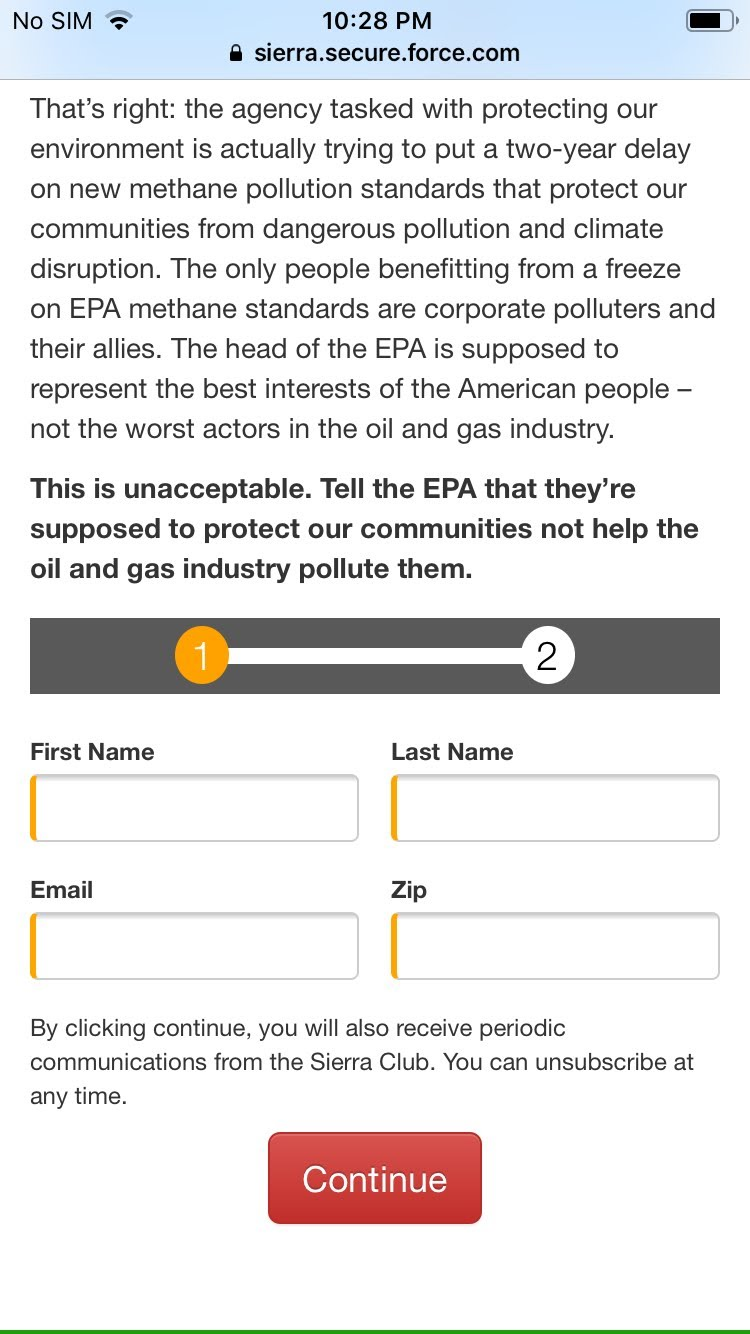
\includegraphics[height = 4in]{Figs/sierra1.jpeg}
    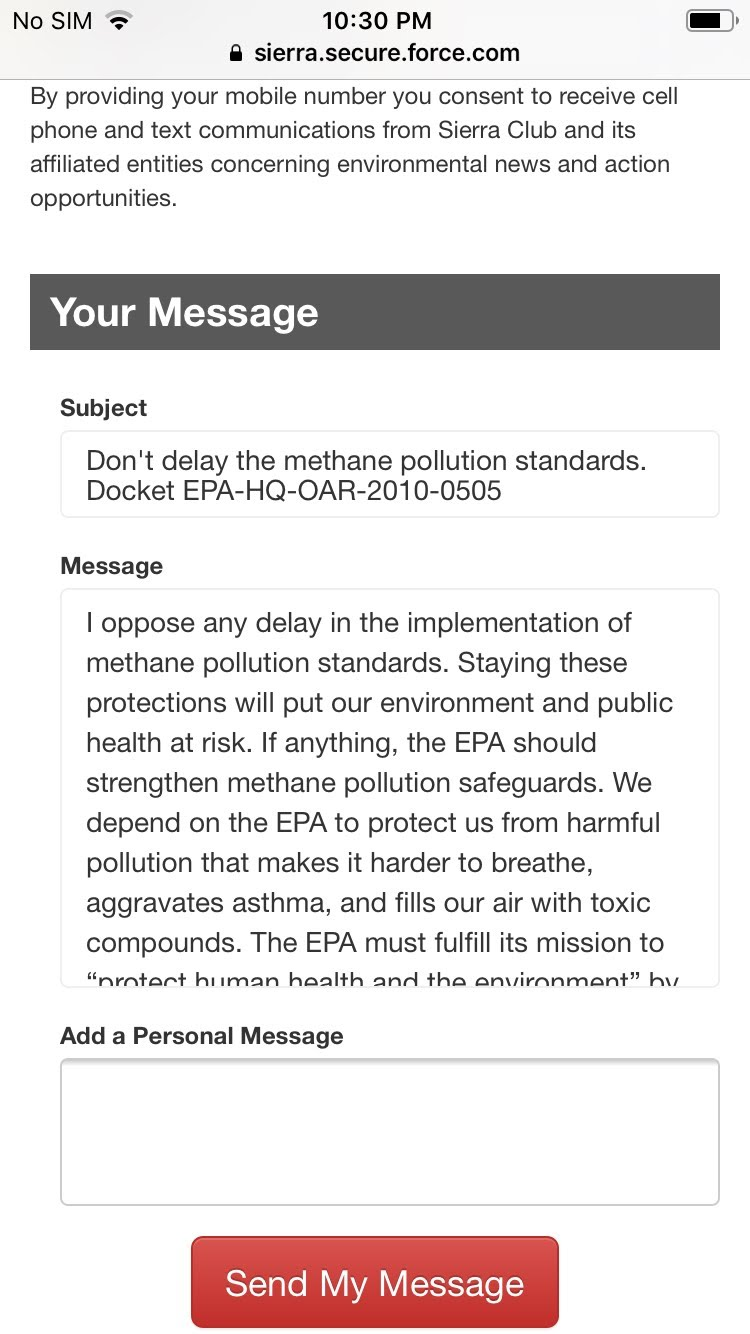
\includegraphics[height = 4in]{Figs/sierra2.jpeg}
    \label{fig:sierra}
\end{figure}

While such campaigns may engage many people, they are unlikely to affect policy or to inspire countermobilization. I expect such campaigns to occur on rules that have high partisan salience (e.g. rules following major legislation passed on a narrow vote), rules that propose large shifts on policy issues dear to well-funded public interest groups, or rules that begun shortly after presidential transitions when executive-branch agendas shift more quickly than public opinion.

\begin{hyp}
When a lobbying coalition with more intense public support successfully mobilizes for reasons other than influencing policy, opposing coalitions with less public support are not more likely to counter-mobilize.
\end{hyp}

Going public and going down fighting may be difficult to in the observed public response. Indeed, members of the public may poorly understand the chances of success. However, groups do likely know their chances of success and will thus invest less in sophisticated insider lobbying under the going down fighting strategy. Table \ref{tab:campaigns-patterns} specifies the general pattern of engaging, that each of the three reasons behind mass-comment campaings suggests. 

% CAMPAIGNS-PATTERNS TABLE 
\begin{table}[t]
\centering 
  \caption{Observable differences in engagement across types of mass-mobilization campaigns}
  \def\arraystretch{1.5}
\begin{tabular}{@{\extracolsep{5pt}} lcccc} 
& Inside &  & Outside &   \\ \cline{3-5} 
& Technical information & Number of comments & Effort & Contagion \\
\hline
Going public & High & High & High & High  \\ 
\hline
Disrupting  & High & Low & Low & Low  \\
\hline
Going down fighting & Low & High & High & High  \\ 
\hline 
\end{tabular}
\end{table}
\label{tab:campaigns-patterns}


% \subsection{Mobilizing for Recruitment}
% A third possibility is that mobilization around bureaucratic decisions is unrelated to the possibility of affecting policy and primarily a way to recruit and engage members or raise the profile of the movement. If this is the case, behaviors like protesting and mass commenting on rules are largely epiphenomena to unrelated kinds of politics. Organizers may know that mobilization has minimal effects, but lead members to engage as a means to other ends. Many of the mobilized themselves may doubt their efficacy but still take advantage of the opportunity to protest. 

While coalitions may form around various material and ideological conflicts, those most likely to be advantaged by going public or going down fighting are public interest groups---organizations primarily serving an idea of the public good rather than the material interests of their members.\footnote{\citet{Berry1999} calls these groups ``citizen groups'' and emphasizes conflict over cultural issues. While some of these groups focus on conservative or progressive cultural issues, like religious education or endangered species, many are more focused on the public provision or protection of public goods such as national parks, consumer product safety standards, air quality, and drinking water, and public safety.

One exception may be the few types of membership organizations that are both broad and focused on material outcomes for their members such as labor unions.} Thus, I theorize that mass mobilization is most likely to occur in conflicts of public versus private interests or public versus public interests (i.e. between coalitions led by groups with distinct cultural ideals or ideas of the public good), provided they have sufficient resources to run a campaign.\footnote{
If true, one implication is that mass mobilization will systematically run counter to concentrated business interests where they conflict with the values of organized, privileged groups.
}

\begin{hyp}
Public interest group coalitions mobilize more often than business-driven coalitions.
\end{hyp}

This hypotheses highlights the conditional logic of mass mobilization. If outside lobbying were purely determined by resources resources, business-driven coalitions would often dominate, as they do elsewhere. However, because outside lobbying alters the decision environment, those advantaged by the usual, more limited set of actors have little incentive to expand the scope of conflict.




% We do not really know who engages in mass commenting. Some assume that people who engage in mass commenting belong to membership organizations. Others imply that they are people who happen to have an opinion. RAUCH discusses both "members" and  _______
% % The people who engage in mass commenting are often assumed to be 

% Engaging a broader audience and thus changing the scope of conflict is a basic political strategy. Presidents, supreme court justices, and others "go public" when doing so alters their opponents' calculations. 

% Which campaigns engage a broader audience and which do not? 


\subsubsection{Patterns of mass engagement} I classify supporters into three types based on how they were mobilized. Comments that are exact copies of a form letter are akin to petition signatures from supporters who were engaged by a campaign to comment with minimal effort. Commenters that also take time to add their own text indicate more intense preferences. Finally, commenters who express solidarity in similar but distinct phrases indicate they were engaged indirectly, perhaps by a news story or a social media post about the campaign, 
as campaign messages spread beyond those originally targeted. Because the success of a mobilization effort is moderated by public support, broader public interest group coalitions ought to mobilize more people, more effort per person, and more people indirectly for the same amount of mobilization effort (e.g. spending or solicitations).  

\begin{hyp}
Public interest group coalitions mobilize more successfully than business-driven coalitions. Indicators of success include (1) the number of comments supporting a coalition (2) the effort per comment (3) the number of comments mobilized indirectly. 
\end{hyp}

\end{subhyp}

The size of each group thus offers political information to policymakers, including coalition resources, the intensity of sentiment, and potential for conflict to spread.
The first two types signal two kinds of intensity or resolve. First, they show the mobilizers' willingness to commit resources to the issue. Second, costly actions show the intensity of opinions among the mobilized segment of the public \citep{Dunleavy1991}. The number of people engaged by a campaign is not strictly proportional to an organizations investment. The less each person care, the more it costs to mobilize them. The third type indicates potential contagion. Indications that messages spread beyond those originally targeted may be especially powerful \citep{Kollman1998}. 

Information about organizational resolve, the intensity of preference, and contagiousness are thus produced, but%, as discuss in section \ref{influence-intro}, 
such political information will only influence decisions if these signals are processed in a way that captures this information and relays it to decisionmakers. These organizational processes may vary significantly across agencies.

The next section outlines 

% better theory
\subsubsection{Incorporating political information into models of lobbying in rulemaking}
% MY THEORY 
% Representation 
When lobbying during rulemaking, groups often make suspect claims to represent broad segments of the public \citep{Seifter2016UCLA}. %Mobilizing a large number of people may support such claims. 
If agency staff do not trust an organizations' representational claims, engaging actual people may be one of the few credible signals of a broad base of support.
% public-private interests 
Appeals to government are almost always couched in the language of public interest, even when true motivations obviously private \citep{Schattschneider1975}. Theorists may debate whether effectively signing a petition of support without having a role in crafting the appeal is a meaningful voice and whether petitions effectively channel public interests, but, at a minimum, engaging a large number of supporters helps distinguish broader interests from truly narrower ones. It suggests the organization is not ``memberless'' \citep{Skocpol2003} in the sense that they are able to demonstrate some verifiable public support.\footnote{
Public support can be faked or inflated using ``astroturf'' tactics but as I argue below, such campaigns ought to have observably different patterns of engagement.}

% tactic
Mass mobilization is a strategy. When successful, mass engagement is the result. An organization's ability to expand the scope of conflict by mobilizing members of the public may occasionally be a valuable political resource. 
In contrast to scholars who focus on the deliberative potential of public comment processes, I focus on public engagement as a tactic aimed at gaining power, either by leveraging powerful ideas or engaging actors with the institutional power to shape decisions.
Scholars who do understand mobilization as a tactic \citep{Furlong1997, Kerwin2011} have thus far focused organizations mobilizing their membership. %In contrast, 
I include a campaign's broader audience and its potential to grow, more akin to the concept of an attentive public \citep{Key1961} or issue public \citep{Converse1964}. If organizations claim to represent people beyond their official members, 
reforms requiring groups to disclose information about their funding and membership \citep{Seifter2016UCLA} only go part way to assess groups' claims to represent these broader segments of the public. Indeed, if advocacy group decisions are largely made by D.C. professionals, these advocates themselves may be unsure how broadly their claims resonate until potentially-attentive publics are actually engaged.
% resource - add David's cite 

% three insights 
Here I build on three insights. First, \citet{Kerwin2011} and \citet{Furlong1997} identify mobilization as a tactic. In their survey, organizations report that forming coalitions and mobilizing large numbers of people are among the most effective lobbying tactics. Second, \citet{Nelson2012} identify political information a potentially influential result of lobbying by different business coalitions. While they focus on mobilizing experts, \citet{Nelson2012} describe a dynamic that can be extended to mass commenting: 
\begin{quote}
``strategic recruitment, we theorize, mobilizes new actors to participate in the policymaking process, bringing with them novel technical and political information. In other words, when an expanded strategy is employed, leaders activate individuals and organizations to participate in the policymaking process who, without the coordinating efforts of the leaders, would otherwise not lobby. This activation is important because it implies that coalition lobbying can generate new information and new actors---beyond simply the `usual suspects'---relevant to policy decision makers. Thus, we theorize consensus, coalition size, and composition matter to policy change.'' 
\end{quote}
I argue that, with respect to political information, this logic extends to non-experts. The number of and distribution of ordinary supporters also matters because it suggests a \textit{public} consensus. Instead of bolstering scientific claims, a perceived public consensus bolsters political claims. 
Third, \citet{Furlong1998}, \citet{Yackee2006JPART}, and others distinguish direct and indirect forms interest group influence in rulemaking. I argue that mass mobilization is a tactic aimed at producing political information.% that may have direct and indirect influence (see section \ref{influence-intro}). 


% PUBLIC OPINION and INFORMATION 
\citet{Rauch2016} suggests that agencies reform the public comment process to include opinion polls. I build from a similar intuition that mass comment campaigns currently function like a poll or, more accurately, a petition, capturing the intensity of preferences among a segment of the public---i.e. how many people are willing to take the time to engage.\footnote{
For example, % public opinion example 
a campaign by the World Wildlife Federation provided language explicitly claiming to have public opinion on their side, their model comment reading ``Along with 80\% of the American people, I strongly support ending commercial trade in elephant ivory in the US.'' This suggests that mass comment campaigns aim to signal information about public opinion.
} 
Self-selection may not be ideal for representation, but opt-in participation---whether voting, attending a hearing, or writing a comment---still provides political information. 
Mobilizing citizens and generating new political information are key functions of interest groups in a democracy \citep{Mansbridge1992, Mahoney2007}. The information generated by mass mobilization campaigns is explicitly political and more complex than an opinion poll. Activists aim to convince people which issues are important and how to think about them---mapping new issues and debates to familiar ones, thereby shifting the political landscape. 

Importantly, rule-specific campaigns inform agencies about the distribution and intensity of opinions that are often too nuanced to estimate a priori. Many rules may lack analogous public opinion polling questions, making mass commenting a unique source of political information. Indeed, as is true about public opinion on many specific policy issues \citep{Hutchings2003},  most members of the public and their elected representatives may only learn about the issue as a result of a mobilization campaign. I thus consider public demands to be a latent factor in my model of policymaking. Public demands shape the decisions of groups who lobby in rulemaking. If they believe the attentive public is on their side, groups may attempt to reveal this political information to policymakers by launching a mass mobilization campaign. The public response to the campaign depends on the extent that the attentive public is passionate about the issue.%\footnote{It is difficult if not impossible to estimate public opinion, much less the intensity of such opinions before people have been made aware of the issue. Occasionally, increased awareness of a policy issue can radically alter its role in politics if a large number of people are given an opportunity to weigh in..."sleeping giants in Hutchings 2003?} 

Figure \ref{fig:causal-whymail} amends the classic model of interest group lobbying to incorporate the above intuitions. In addition to providing technical information, for example through sophisticated comments, an organization may mobilize supporters. The broader and more intense support the group has, the more successful this effort will be. Large-scale engagement may produce several types of relevant political information. The most direct and obvious is the expressed ``public opinion'' that policymakers observe.\footnote{I address other types of political information that mass engagement may create elsewhere. For an expanded model, see Figure \ref{fig:causal-full} in the Appendix.}

\begin{figure}[h!]
    \centering
    \caption{Incorporating Mass Engagement and Political Information into Models of Lobbying}
    \label{fig:causal-whymail}
\tiny
\begin{tikzpicture}[%
    node distance=1.2cm,
    auto,
    text width=1.5cm,
dnode/.style={diamond, align=center, aspect=2, fill=green!5,draw=green!60, very thick, minimum size=2cm},
squarednode/.style={rectangle, align=center, aspect=1, draw=red!60, fill=red!5, very thick, minimum size=1cm},
pnode/.style={ellipse, align=center, aspect=1, draw=black!60, fill=black!5, very thick, minimum size=1cm},
title/.style={rectangle, align=center, aspect=1, minimum size=2cm},
]
% Draft 
\node[dnode]      (draft)                     {Draft Policy};



% Group Nodes
\node[pnode]      (groupdemands) [right=of draft] {Group Demands};
\node[dnode]        (groupdecides) [right=of groupdemands] {Lobbying Strategy};
\node[squarednode]      (groupinfo) [right=of groupdecides] {Technical Information};

% policy 
\node[dnode]      (policy)       [right=of groupinfo] {Policy Response};
\draw[->] (groupinfo.east) -- (policy.west);
% \draw[->] (publicinfo.east) -- (policy.west);
% \draw[->] (principalinfo.east) -- (policy.south);
% \draw[->] (principalinfo2.east) -- (policy.south);

% Group Lines
\draw[->] (draft.east) -- (groupdemands.west);
\draw[->] (groupdemands.east) -- (groupdecides.west);
\draw[->] (groupdecides.east) -- (groupinfo.west);

% Titles
% \node[title]      (1) [above=of draft] {Policy};
% \node[title]      (2) [above=of groupdemands] {Preferences};
% \node[title]      (4) [above=of groupinfo] {Information/ Signal};
% \node[title]      (3) [above=of groupdecides] {Observed Behavior};
% \node[title]      (5) [above=of policy] {Policy'};

% political info
\node[rectangle, minimum width =2cm, minimum height = 3cm, draw=red!60, fill=red!5, very thick]      (politicalinfo) [below=of groupinfo] {};
\node[text centered]      (politicalinfotext) [below=of groupinfo] {Political Information};
\node[text centered]      (mobilizing) [below=of groupdecides] {Mass\\ Mobilization};
\draw[->] (politicalinfo.north east) -- (policy.south west);

% public Nodes
\node[squarednode]      (publicinfo) [below=of politicalinfotext] {Perceived ``Public'' Opinion};
\node[dnode]      (publicdecides) [left=of publicinfo] {Mass\\ Engagement};
\node[pnode]        (publicdemands) [left=of publicdecides] {Latent Public Demands};

% public Lines
% \draw[->] (draft.east) -- (publicdemands.west);
\draw[->] (publicdemands.east) -- (publicdecides.west);
\draw[->] (publicdemands.north east) -- (groupdecides.south west);
\draw[-] (groupdecides.south) -- (mobilizing.north);
\draw[->] (mobilizing.south) -- (publicdecides.north);
\draw[->] (publicdecides.east) -- (publicinfo.west);



\end{tikzpicture}
\end{figure}
\normalsize

The causal process visualized in figure \ref{fig:causal-whymail} only operates under certain conditions. 
As suggested above, one of those conditions is that mobilization was aimed at influencing policy. 
% As I will describe in section \ref{influence-intro}, another condition is that agencies have the capacity to process political information. 
%But first, section \ref{principals-intro} focuses on another key source of political information: political oversight behavior.
% Another condition is that the ...This latter condition is key to the present question of why mass engagement occurs.
% In order to answer this question, we need a theory why mass commenting occurs and systematic analysis of public commenting behavior in agency rulemaking. 
